\documentclass{article}
\usepackage{graphicx} % Required for inserting images
\usepackage{blindtext}
\usepackage{hyperref}
\usepackage[a4paper]{geometry}
\geometry{left=2cm,right=2cm,vmargin=2cm}
\pagestyle{plain}


\title{LEPL1110 - Rapport sur les déformations d'un avion}
\author{Groupe 55 : Targonski Krystian, 42942000 - Ulysse Reinbold, 30522000}
\date{Avril 2024}

\begin{document}

\maketitle

\section{Description du problème}
    Notre projet vise à clarifier une chose importante : les avions sont en fait assez solides. Beaucoup de personnes se posent des questions sur l'intégrité des ailes lorsque celles-ci se déforment au décollage ou même en cours de vol. Ce que nous allons vérifer ici, c'est que ce genre de déformations est tout à fait acceptable et même normal. Pour cela, nous avons effectué une modélisation d'un avion (voir Fig.\ref{fig:mesh_mauve}) et avons observé comment les ailes se déforment en fonction de la vitesse, de l'altitude et aussi de la masse que l'avion transporte à un moment donné. Voici une représentation du problème avec le maillage que nous avons créé :
    \begin{center}
        \begin{figure}[h]
            \centering
            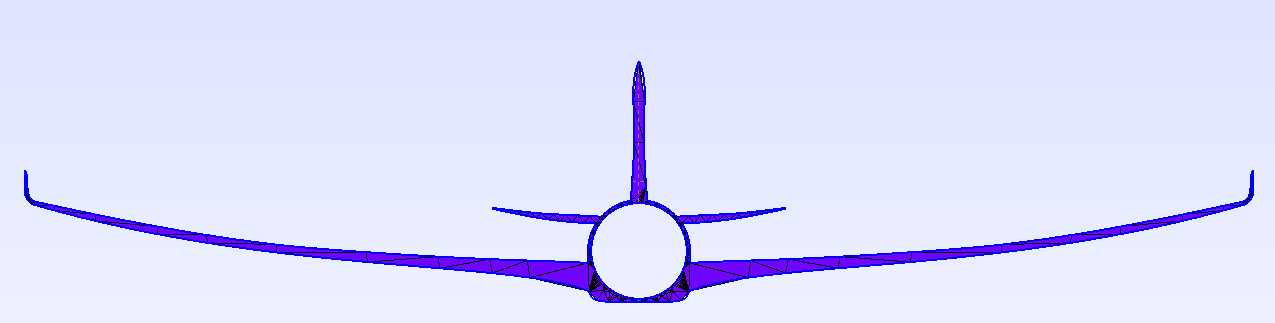
\includegraphics[scale=0.3]{Screenshot from 2024-04-12 15-27-26.png}
            \caption{Mesh}
            \label{fig:mesh_mauve}
        \end{figure}
    \end{center}

    Nous avons également établi quelques hypothèses pour simplifier cette situation en un problème d'élasticité en 2D réalisable. Les voici : 
    \begin{itemize}
        \item Les déformations qui nous intéressent se produisent uniquement selon l'axe des Y (haut/bas) sur notre plan.
        \item La portance est générée exclusivement par les ailes.
        \item D'un point de vue un peu plus réaliste, nous avons choisi de nous baser sur un avion existant, l'Airbus A350-900. Toutes nos valeurs sont donc tirées des informations disponibles sur cet avion (principalement sur le site d'Airbus et Wikipédia).
        \item Par simple curiosité, nous avons décidé de modifier la composition du fuselage. En réalité, il est composé à moitié de matériaux composites, tels que la fibre de carbone, ainsi que d’un mélange d'alliages d'aluminium et de titane. Cependant, nous avons décidé d'observer ce qui se passe si tout l'avion était fabriqué à 100\% de fibres de carbone, comme les ailes.
\end{itemize}
    
\section{Physique du problème}
    Suivant ces hypothèses, notre avion ne subit que deux forces lors de son vol : la première est la portance, et la seconde est son poids. La force de portance est appliquée sur les deux ailes, ce qui implique un moment de force sur celles-ci et donc une déformation. Nous n'allons pas nous attarder beaucoup sur ce point, mais voici la formule que nous avons utilisée pour calculer la portance de nos ailes :

\[F = \frac{k}{2} * \rho * V^2 * S\]

Avec :
    \begin{itemize}
        \item \(k\), qui est une constante dépendante de la forme de l'aile, typiquement comprise entre 0.3 et 0.7. Pour notre application, nous avons découvert qu'elle vaut 0.38.
        \item \(\rho\), qui est la masse volumique de l'air.
        \item \(V\), qui est la vitesse de l'avion. Dans des conditions de vol standards, elle est de Mach 0.85.
        \item \(S\), qui est la surface de portance. Dans notre cas, elle est de 443 m².
    \end{itemize}
    Pour compléter ces informations et bien définir le problème, voici les caractéristiques des \href{https://gernitex.com/fr/ressources/fibre-de-carbone-proprietes/} {ailes} :
    \begin{itemize}
        \item Module d'élasticité : 294 GPa
        \item Élongation maximale : 1.75\%
        \item Résistance à la traction : 5407 MPa
    \end{itemize}

    
\section{Résolution du problème}
La partie un peu plus intéressante maintenant : pour résoudre ce problème, nous avons implémenté un solveur CG + CSR qui nous a permis de simuler différents scénarios sur notre maillage (il convient de préciser qu'il est également bien plus rapide ! D'après nos tests, CS + CSR est environ 45 fois plus rapide que le solveur fourni par défaut ! Un temps de calcul moyen de 12.9 s est descendu à 0.29 ms).

Tout d'abord, nous avons dû mettre en place des conditions aux limites de manière à ce que le modèle : 1) ne se casse pas directement ou ne réalise pas des mouvements inattendus, et 2) que les mouvements de déformation soient bien ceux que nous voulons analyser. Pour cela, nous avons utilisé une combinaison de conditions de Dirichlet et de Neumann sur les parties les plus susceptibles de se déformer : le bas du fuselage ainsi que le haut, les winglets au bout des ailes, et bien évidemment les ailes. De toutes ces parties, seules les ailes sont libres de bouger suivant les forces qui s'appliquent dessus ; les wingtips sont fixés à suivre les ailes, et le fuselage en général est rempli de conditions de Dirichlet pour éviter tout mouvement sporadique.


\section{Résultats et interprétation}
À part quelques situations inattendues (voir Fig.\ref{fig:mesh_rigolo}) dues à des valeurs un peu trop élevées des forces, nous avons observé une déformation acceptable de l'ordre de 5 mètres en hauteur, en fonction de la charge que transporte l'avion. Ceci correspond aux données fournies par Airbus. Pour visualiser cette déformation de manière plus illustrative, voici une petite \href{https://drive.google.com/file/d/1oQy1q5MK8c4jTr_zF4XT-4oIqpgq1oaf/view?usp=drive_link}{animation}\footnote{\texttt{https://drive.google.com/file/d/1oQy1q5MK8c4jTr\_zF4XT-4oIqpgq1oaf/view?usp=drive\_link}}. Une observation assez importante est la nette augmentation du stress au niveau de la connexion entre le fuselage et les ailes lorsque la charge augmente. Ce phénomène peut en effet représenter un comportement dangereux pour ces matériaux. Cependant, il est important de préciser que nous avons dû augmenter à \href{https://drive.google.com/file/d/1oRUz1sT_RANzSDQ2jbQxheanYzACV3mM/view?usp=drive_link}{100 tones}\footnote{\texttt{https://drive.google.com/file/d/1oRUz1sT\_RANzSDQ2jbQxheanYzACV3mM/view?usp=drive\_link}} au-dessus de la limite de chargement autorisée par Airbus pour cet avion.
\begin{figure}[h]
  \centering
  \begin{minipage}[h]{0.4\textwidth}
    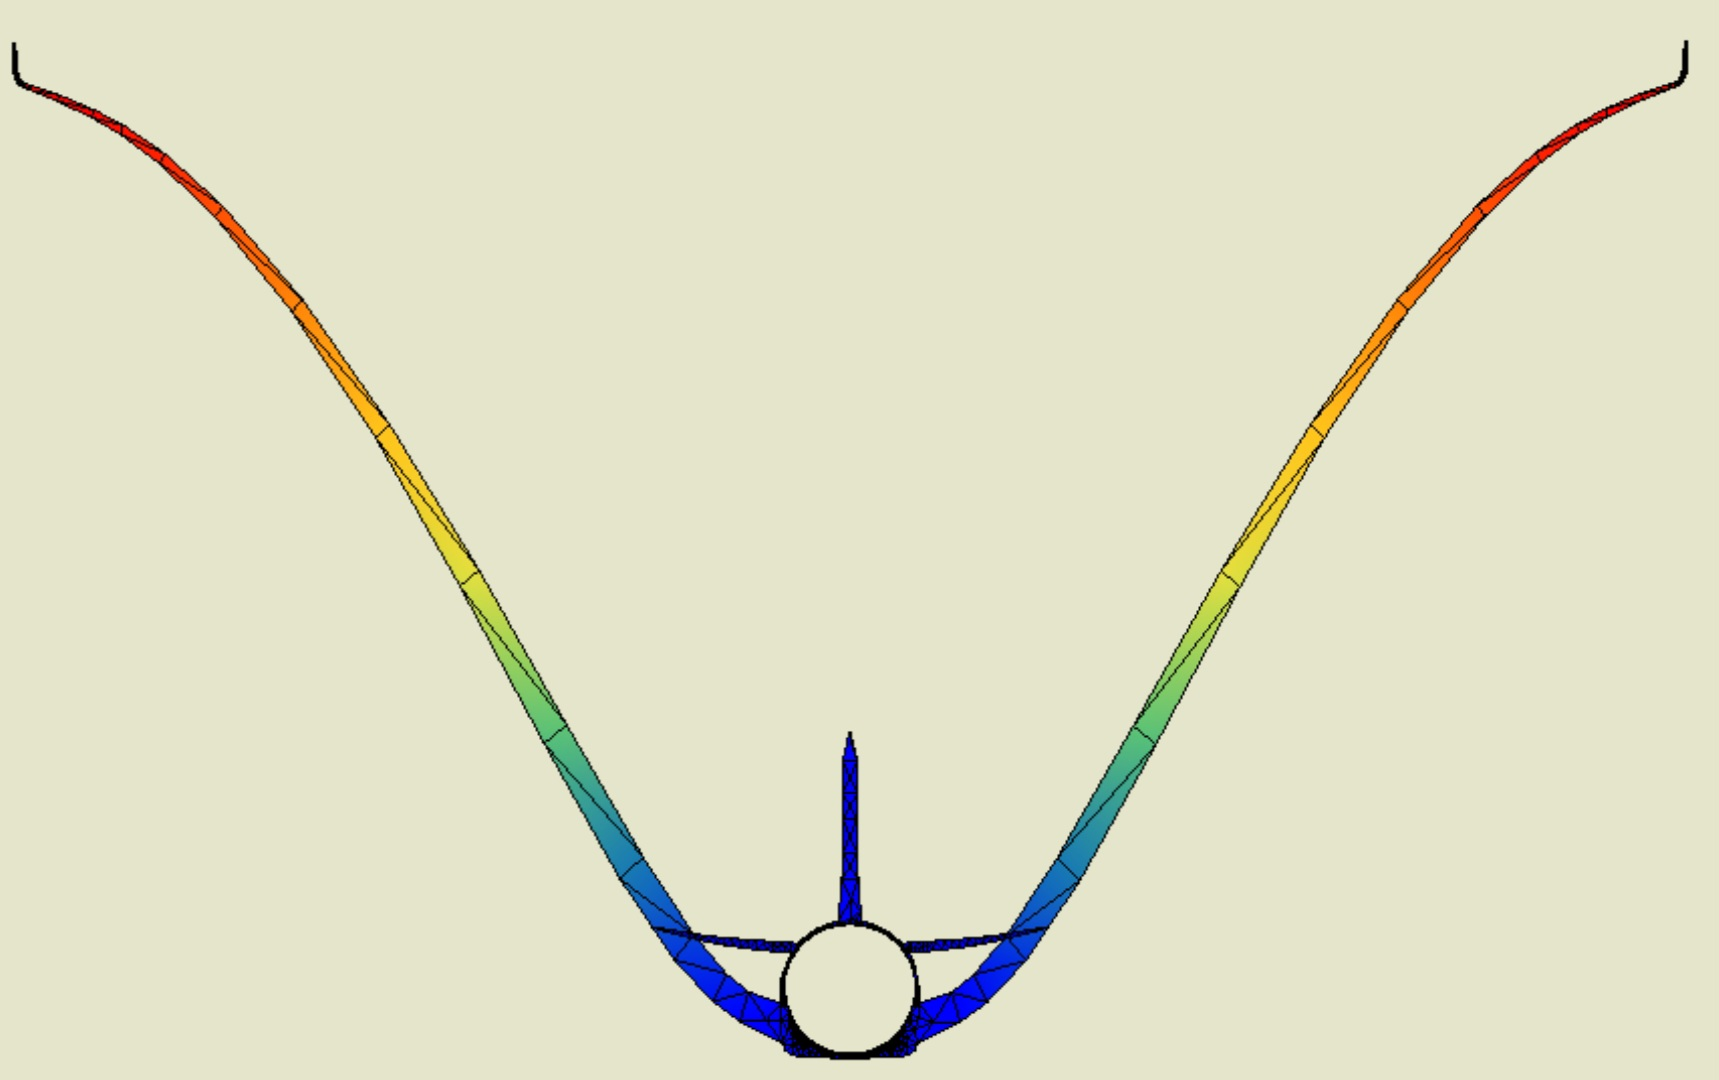
\includegraphics[scale=0.11]{udef.jpg}
    \caption{Mesh Rigolo}
    \label{fig:mesh_rigolo}
  \end{minipage}
  \hfill
  \begin{minipage}[h]{0.4\textwidth}
    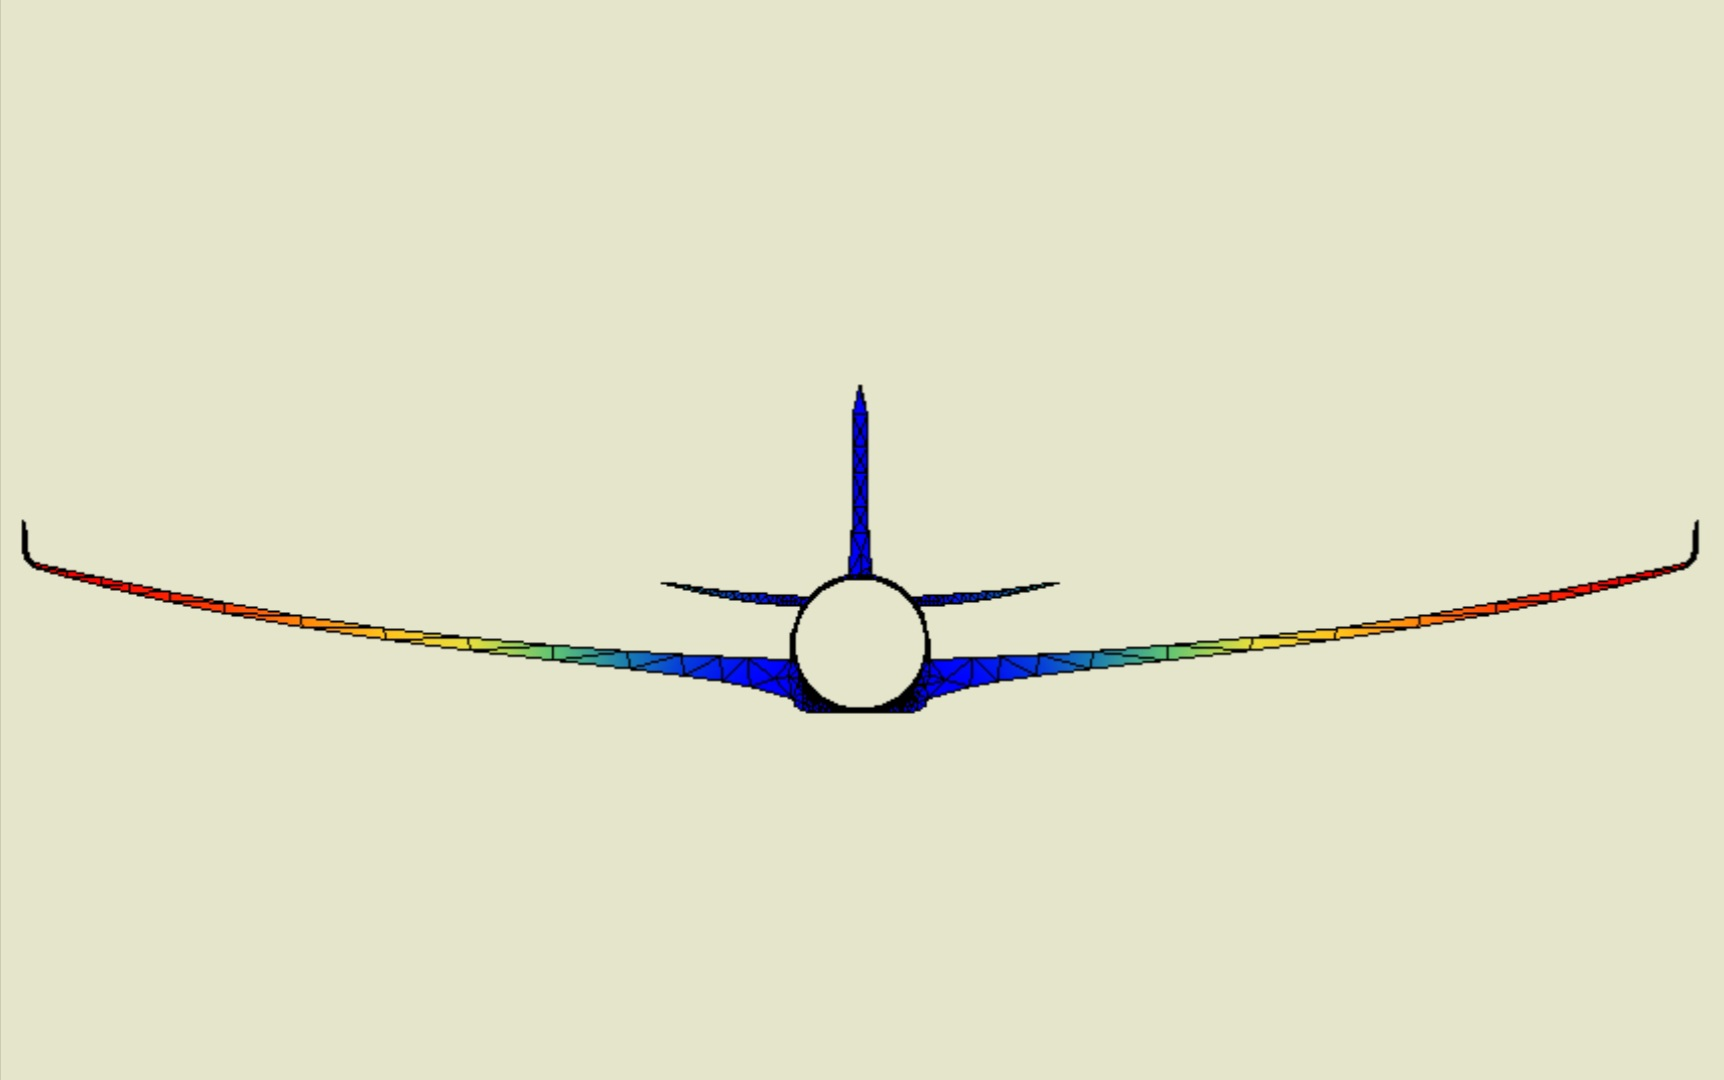
\includegraphics[scale=0.11]{normal_def.jpg}
        \caption{Déformation normale}
        \label{fig:mesh_normal}
  \end{minipage}
\end{figure}

Le mouvement naturel des ailes est clairement observable et ne soulève pas de préoccupations à moins de dépasser les limites fixées, au-delà desquelles des signes de fissures pourraient apparaître. Il est donc normal que les ailes bougent pendant le vol.

En vol, la vitesse de l'air est variable, ce qui soulève la question de son impact sur la déformation des ailes, étant donné que la vitesse influence la portance. Bien que les fluctuations de vitesse ne provoquent pas de changement significatif, la déformation devient plus visible à mesure que la vitesse de l'avion augmente.

Enfin, bien que le changement d'altitude puisse avoir une influence indirecte sur la portance, son impact sur la déformation des ailes est négligeable.


\end{document}
